\chapter{模块3(实验与分析)}

\section{创新思想和学术贡献}

在本文中,我们提出了一种基于凸基学习器的元学习方法,用于少样本学习。
对偶形式和KKT条件可用于实现计算和存储效率高的元学习,特别适用于少样本学习问题。
与最近邻分类器相比,线性分类器在稍微增加计算成本的情况下提供更好的泛化能力。
我们的实验表明,正则化的线性模型允许更高的嵌入维度,并减少了过度拟合。对于未来的工作,
我们旨在探索其他凸基学习器,如核SVM。这将允许随着更多的训练数据可用于任务而逐渐增加模型容量的能力。

\section{实验方法}
我们首先描述了在实验中使用的网络架构和优化细节。
然后,我们展示了在标准的几种少样本分类基准上的结果,包括ImageNet的派生数据集和CIFAR,
随后使用相同的嵌入网络和训练设置对各种基础学习器对准确性和速度的影响进行了详细分析。
\subsection{实验细节}
元学习设置。我们在实验中使用了一个ResNet-12网络,遵循\cite{oreshkin2018tadam,mishra2017simple}。
令Rk表示由三个{3×3卷积和k个滤波器,批归一化,Leaky ReLU(0.1)}组成的残差块;令MP表示2×2最大池化。我们使用了DropBlock正则化\cite{ghiasi2018dropblock},
一种结构化Dropout形式。令DB(k,b)表示具有保持率为k和块大小为b的DropBlock层。
用于ImageNet衍生数据集的网络架构为:R64-MP-DB(0.9,1)-R160-MP-DB(0.9,1)-R320-MP-DB(0.9,5)-R640-MP-DB(0.9,5),
而用于CIFAR衍生数据集的网络架构为:R64-MP-DB(0.9,1)-R160-MP-DB(0.9,1)-R320-MP-DB(0.9,2)-R640-MP-DB(0.9,2)。
在最后的残差块后,我们不应用全局平均池化。

作为优化器,我们使用带有0.9的Nesterov动量和0.0005的权重衰减的SGD。
每个小批次包含8个样本集。该模型进行了60个epochs的元训练,每个epoch包含1000个样本集。
学习率最初设置为0.1,然后在第20、40和50个epoch时分别更改为0.006、0.0012和0.00024,这是遵循\cite{gidaris2018dynamic}的实践。

在元训练期间,我们采用了水平翻转、随机裁剪和颜色(亮度、对比度和饱和度)扰动数据增强,如\cite{gidaris2018dynamic,qiao2018few}中所述。
对于使用ResNet-12的miniImageNet实验,我们使用eps = 0.1的标签平滑。与\cite{snell2017prototypical}使用元训练的高路径分类不同,
我们在两个阶段都使用5路分类,这是遵循最近的工作\cite{gidaris2018dynamic,oreshkin2018tadam}。每个类别在元训练期间包含6个测试(查询)样本,
在元测试期间包含15个测试样本。我们的元训练模型是基于元验证集上5路5-shot测试准确性选择的。

对于原型网络,我们将元训练shot设置为与元测试shot相匹配,这是遵循通常的做法\cite{snell2017prototypical,gidaris2018dynamic}。
对于SVM和岭回归,我们观察到保持元训练shot高于元测试shot可以获得更好的测试准确性,如 图\ref{fig:2} 所示。因此,在元训练期间,
我们针对ResNet-12的miniImageNet将训练shot设置为15;对于使用4层CNN的miniImageNet(在表\ref{table:3}中)将训练shot设置为5;
对于tieredImageNet,将训练shot设置为10;对于CIFAR-FS,将训练shot设置为5;对于FC100,将训练shot设置为15。

\begin{figure}[htbp]
    \centering
    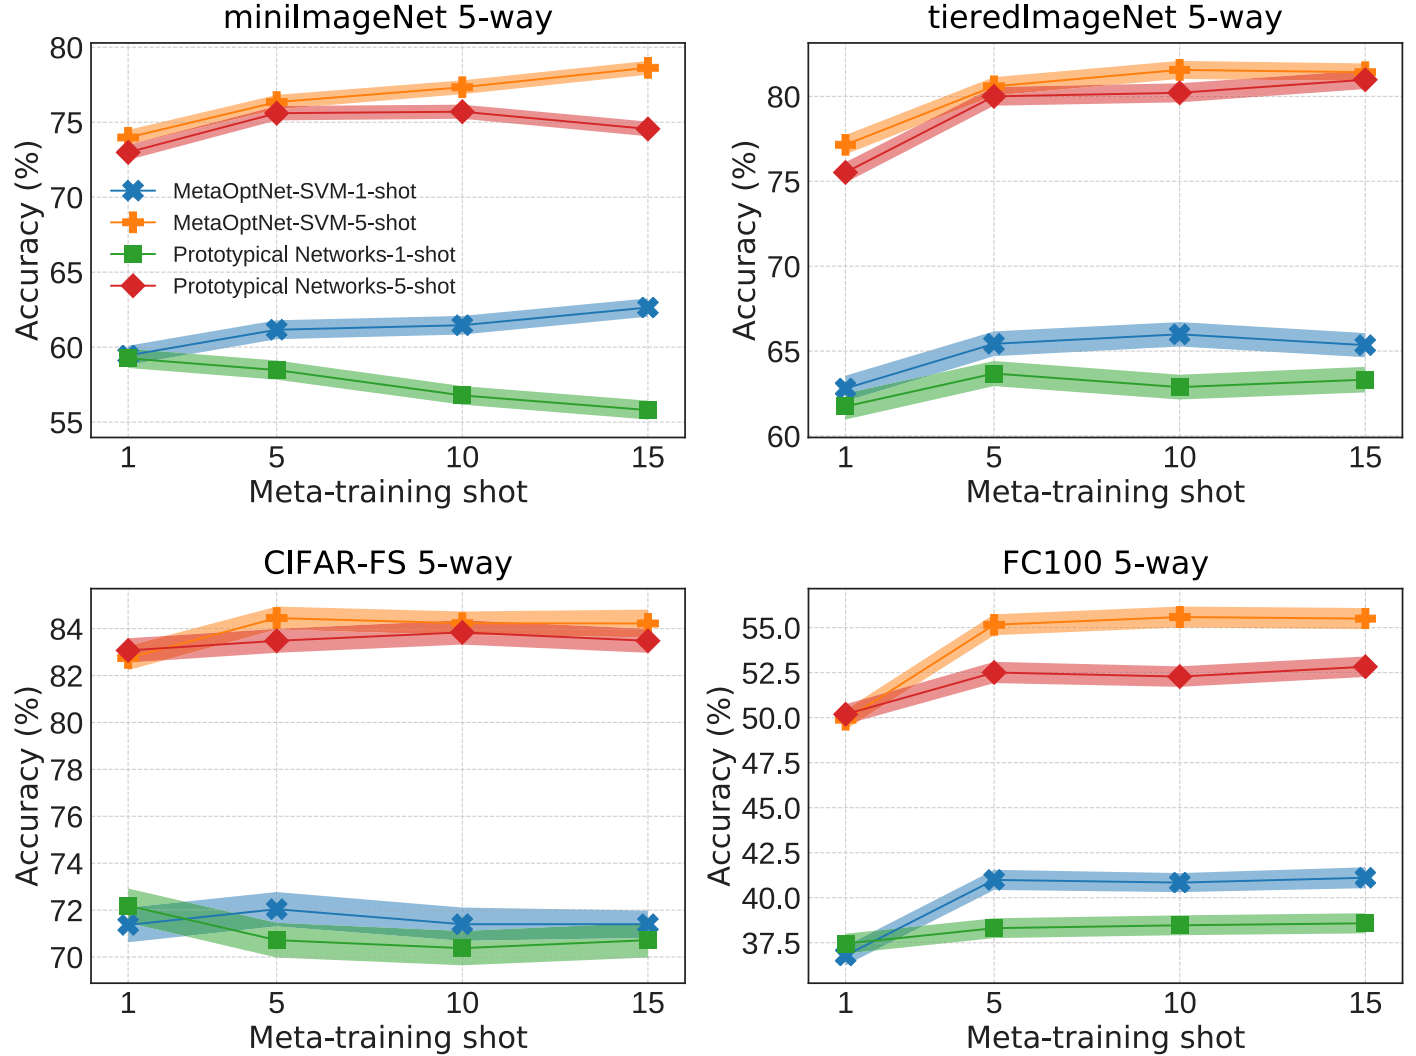
\includegraphics[width=.7\linewidth]{figure/f2.png}
    \caption{使用不同的元训练样本数量,在miniImageNet元测试集上的测试准确率(\%)。}
    \label{fig:2}
\end{figure}

基学习器的设置。对于线性分类器的训练,我们使用二次规划求解器OptNet \cite{amos2017optnet}。
SVM的正则化参数C设置为0.1。岭回归的正则化参数λ设置为50.0。对于最近类均值(原型网络),
我们使用针对特征维度进行归一化的平方欧几里得距离。

提前停止。虽然我们可以运行优化器直到收敛,但在实践中,我们发现在固定的迭代次数(仅三次)
内运行QP求解器实际上效果很好。提前停止起到了额外的正则化作用,甚至可以带来稍微更好的性能。


\subsection{在ImageNet的衍生数据集上的实验}

miniImageNet数据集\cite{vinyals2016matching}是用于少样本图像分类的标准基准测试,
由ILSVRC-2012 \cite{russakovsky2015imagenet}中随机选择的100个类组成。
这些类别随机分为64、16和20个类别,用于元训练、元验证和元测试。每个类别包含大小为84×84的600张图像。
由于原始出版物\cite{vinyals2016matching}中未公布类别分割,因此我们使用了\cite{ravi2017optimization}中提出的常用分割。

tieredImageNet基准测试\cite{ren2018meta}是ILSVRC-2012 \cite{russakovsky2015imagenet}的一个较大子集,由608个类别组成,分为34个高级类别。
这些类别分为20个类别用于元训练,6个类别用于元验证,8个类别用于元测试。这相当于元训练、元验证和元测试分别有351、97和160个类别。
该数据集旨在最小化分割之间的语义相似性。所有图像的大小均为84×84。

结果。表\ref{table:1}总结了5-way miniImageNet和tieredImageNet上的结果。在miniImageNet和tieredImageNet元测试集上,
使用95\%置信区间的平均few-shot分类准确率(\%)。“a-b-c-d”表示每个层中具有a,b,c和d个滤波器的4层卷积网络。
†表示使用元训练集和元验证集的并集来元训练元学习器。“RR”代表岭回归。
\begin{table}[htbp]
    \resizebox{\linewidth}{!}{  

    \begin{tabular}{
    l 
    l 
    c 
    c 
    l 
    l }
    \toprule 
                                                     &                                   & \multicolumn{2}{c}{\textbf{miniImageNet 5-way}}                                                               & \multicolumn{2}{c}{\textbf{tieredImageNet 5-way}}                                                 \\ \cline{3-6} 
    \textbf{model}                                   & \textbf{backbone}                 & \textbf{1-shot}                                                   & \textbf{5-shot}                                                   & \multicolumn{1}{c}{\textbf{1-shot}} & \multicolumn{1}{c}{\textbf{5-shot}} \\ \hline
    Meta-Learning LSTM*                              & 64-64-64-64                       & 43.44 ± 0.77                                                      & 60.60 ± 0.71                                                      & -                                                           & -                                                           \\
    Matching Networks*                               & 64-64-64-64                       & 43.56 ± 0.84                                                      & 55.31 ± 0.73                                                      & -                                   & -                                   \\
    MAML                                             & 32-32-32-32                       & 48.70 ± 1.84                                                      & 63.11 ± 0.92                                                      & 51.67 ± 1.81                                                & 70.30 ± 1.75                                                \\
    Prototypical Networks*                           & 64-64-64-64                       & 49.42 ± 0.78                                                      & 68.20 ± 0.66                                                      & 53.31 ± 0.89                                                & 72.69 ± 0.74                                                \\
    Relation Networks*                               & 64-96-128-256                     & 50.44 ± 0.82                                                      & 65.32 ± 0.70                                                      & 54.48 ± 0.93                                                & 71.32 ± 0.78                                                \\
    R2D2                                             & 96-192-384-512                    & 51.2 ± 0.6                                                        & 68.8 ± 0.1                                                        & -                                   & -                                   \\
    Transductive Prop Nets                           & 64-64-64-64                       & 55.51 ± 0.86                                                      & 69.86 ± 0.65                                                      & 59.91 ± 0.94                                                & 73.30 ± 0.75                                                \\
    SNAIL                                            & ResNet-12                         & 55.71 ± 0.99                                                      & 68.88 ± 0.92                                                      & -                                   & -                                   \\
    Dynamic Few-shot                                 & 64-64-128-128                     & 56.20 ± 0.86                                                      & 73.00 ± 0.64                                                      & -                                   & -                                   \\
    AdaResNet                                        & ResNet-12                         & 56.88 ± 0.62                                                      & 71.94 ± 0.57                                                      & -                                   & -                                   \\
    TADAM                                            & ResNet-12                         & 58.50 ± 0.30                                                      & 76.70 ± 0.30                                                      & -             -                                   \\
    Activation to Parameter† & WRN-28-10                         & 59.60 ± 0.41                                                      & 73.74 ± 0.19                                                      & -                                   & -                                   \\
    LEO                                              & WRN-28-10                         & 61.76 ± 0.08                                                      & 77.59 ± 0.12                                                      & 66.33 ± 0.05                                                & 81.44 ± 0.09                                                \\
    MetaOptNet-RR (ours)                             & ResNet-12 & 61.41 ± 0.61                                                      & 77.88 ± 0.46                                                      & \textbf{65.36 ± 0.71}                                       & \textbf{81.34 ± 0.52}                                       \\
    MetaOptNet-SVM (ours)                            & ResNet-12                         & 62.64 ± 0.61                                                      & 78.63 ± 0.46                                                      & \textbf{65.99 ± 0.72}                                       & \textbf{81.56 ± 0.53}                                       \\
    MetaOptNet-SVM-trainval (ours)†                  & ResNet-12                         & \textbf{64.09 ± 0.62} & \textbf{80.00 ± 0.45} & \textbf{65.81 ± 0.74}                                       & \textbf{81.75 ± 0.53}                                       \\
    \bottomrule
    \end{tabular}
    }
    \caption{与之前在miniImageNet和tieredImageNet上的工作进行比较}
    \label{table:1}
\end{table}
我们的方法在5-way miniImageNet和tieredImageNet基准测试上取得了最先进的性能。
请注意,LEO \cite{rusu2018meta}除了使用WRN-28-10主干网络外,还利用编码器和关系网络来产生梯度下降的样本相关初始化。
TADAM \cite{oreshkin2018tadam}为每个卷积层使用任务嵌入网络(TEN)块,用于预测元素级比例和偏移向量。

我们还注意到,\cite{rusu2018meta,qiao2018few}对WRN-28-10特征提取器\cite{zagoruyko2016wide}进行预训练,以共同分类miniImageNet元训练集中的全部64个类别;然后在元训练期间冻结网络。
\cite{oreshkin2018tadam}使用了一种类似的策略,使用标准分类任务:他们同时在few-shot分类任务(5-way)和标准分类任务(64-way)上联合训练特征嵌入。
相比之下,我们的系统是端到端进行元训练的,明确地训练特征提取器在带有正则化线性分类器的few-shot学习任务上表现良好。
这种策略允许我们清晰地看到元学习的效果。我们的方法可能更简单,但实现了强大的性能。

\subsection{CIFAR派生数据集的实验}

CIFAR-FS数据集\cite{bertinetto2018meta}是最近提出的few-shot图像分类基准测试,
由CIFAR-100 \cite{krizhevsky2010cifar}中的全部100个类别组成。这些类别被随机分为64、16和20个类别用于元训练、元验证和元测试。每个类别包含大小为32×32的600张图像。

FC100数据集\cite{oreshkin2018tadam}是另一个源自CIFAR-100 \cite{krizhevsky2010cifar}的数据集,包含100个类别,这些类别被分成20个超类。这些类别被划分为60个来自12个超类的类别,
用于元训练,20个来自4个超类的类别用于元验证,以及20个来自4个超类的类别用于元测试。目标是最小化类别之间的语义重叠,
类似于tieredImageNet的目标。每个类别包含大小为32×32的600张图像。

结果。表\ref{table:2}总结了5-way分类任务的结果,我们的MetaOptNet-SVM方法实现了最先进的性能。在更难的FC100数据集上,
各种基学习器之间的差距更为显著,这突显了复杂基学习器在few-shot学习设置中的优势。

\begin{table}[htbp]
    \resizebox{\linewidth}{!}{  
    \begin{tabular}{llcccc}
    \hline
                                    &                   & \multicolumn{2}{c}{\textbf{CIFAR-FS 5-way}} & \multicolumn{2}{c}{\textbf{FC100 5-way}}                      \\ \hline
    \textbf{model}                  & \textbf{backbone} & \textbf{1-shot}      & \textbf{5-shot}      & \textbf{1-shot}     & \textbf{5-shot}                         \\ \hline
    MAML*                           & 32-32-32-32       & 58.9 ± 1.9           & 71.5 ± 1.0           & -                   & -                                       \\
    Prototypical Networks*†         & 64-64-64-64       & 55.5 ± 0.7           & 72.0 ± 0.6           & 35.3 ± 0.6          & 48.6 ± 0.6                              \\
    Relation Networks*              & 64-96-128-256     & 55.0 ± 1.0           & 69.3 ± 0.8           & -                   & -                                       \\
    R2D2                            & 96-192-384-512    & 65.3 ± 0.2           & 79.4 ± 0.1           & -                   & -                                       \\
    TADAM                           & ResNet-12         & -                    & -                    & 40.1 ± 0.4          & 56.1 ± 0.4                              \\
    ProtoNets (our backbone)        & ResNet-12         & \textbf{72.2 ± 0.7}  & 83.5 ± 0.5           & 37.5 ± 0.6          & 52.5 ± 0.6                              \\
    MetaOptNet-RR (ours)            & ResNet-12         & \textbf{72.6 ± 0.7}  & \textbf{84.3 ± 0.5}  & 40.5 ± 0.6          & 55.3 ± 0.6                              \\
    MetaOptNet-SVM (ours)           & ResNet-12         & \textbf{72.0 ± 0.7}  & \textbf{84.2 ± 0.5}  & 41.1 ± 0.6          & 55.5 ± 0.6                              \\
    MetaOptNet-SVM-trainval (ours)¶ & ResNet-12         & \textbf{72.8 ± 0.7}  & \textbf{85.0 ± 0.5}  & \textbf{47.2 ± 0.6} & \multicolumn{1}{l}{\textbf{62.5 ± 0.6}} \\ \hline
    \end{tabular}
    }
    \caption{在不同的元训练样本量下,miniImageNet元测试集的测试准确率(以百分比表示)}
    \label{table:2}
\end{table}

\section{实验结果比较}

表\ref{table:3}显示了我们改变两种不同嵌入架构的基学习器后的结果。当我们使用标准的4层卷积网络,特征维度较低(1600)时,
我们没有观察到采用判别式分类器对few-shot学习的实质性益处。事实上,最近邻类均值分类器\cite{mensink2013distance}在低维特征下表现良好,
如Prototypical Networks\cite{sung2018learning}所示。
然而,当嵌入维度远高于16000时,SVM比其他基学习器产生更好的few-shot准确性。因此,当高维特征可用时,正则化线性分类器提供了鲁棒性。

\begin{table}[htbp]
    \resizebox{\linewidth}{!}{  
    \begin{tabular}{lcccccccc}
    \hline
                          & \multicolumn{4}{c}{\textbf{miniImageNet 5-way}}                                    & \multicolumn{4}{c}{\textbf{tieredImageNet 5-way}}                                 \\ \cline{2-9} 
                          & \multicolumn{2}{c}{\textbf{1-shot}}      & \multicolumn{2}{c}{\textbf{5-shot}}     & \multicolumn{2}{c}{\textbf{1-shot}}     & \multicolumn{2}{c}{\textbf{5-shot}}     \\
    \textbf{model}        & \textbf{acc. (\%)}  & \textbf{time (ms)} & \textbf{acc. (\%)}  & \textbf{ime (ms)} & \textbf{acc. (\%)}  & \textbf{ime (ms)} & \textbf{acc. (\%)}  & \textbf{ime (ms)} \\ \hline
    \multicolumn{9}{l}{\textbf{4-layer conv (feature dimension=1600)}}                                                                                                                             \\
    Prototypical Networks & 53.47±0.63          & 6±0.01             & 70.68±0.49          & 7±0.02            & 54.28±0.67          & 6±0.03            & 71.42±0.61          & 7±0.02            \\
    MetaOptNet-RR (ours)  & 53.23±0.59          & 20±0.03            & 69.51±0.48          & 27±0.05           & 54.63±0.67          & 21±0.05           & 72.11±0.59          & 28±0.06           \\
    MetaOptNet-SVM (ours) & 52.87±0.57          & 28±0.02            & 68.76±0.48          & 37±0.05           & 54.71±0.67          & 28±0.07           & 71.79±0.59          & 38±0.08           \\ \hline
    \multicolumn{9}{l}{\textbf{ResNet-12 (feature dimension=16000)}}                                                                                                                               \\
    MetaOptNet-SVM (ours) & 59.25±0.64          & 60±17              & 75.60±0.48          & 66±17             & 61.74±0.77          & 61±17             & 80.00±0.55          & 66±18             \\
    MetaOptNet-RR (ours)  & 61.41±0.61          & 68±17              & \textbf{77.88±0.46} & 75±17             & \textbf{65.36±0.71} & 69±17             & \textbf{81.34±0.52} & 77±17             \\
    MetaOptNet-SVM (ours) & \textbf{62.64±0.61} & 78±17              & \textbf{78.63±0.46} & 89±17             & \textbf{65.99±0.72} & 78±17             & \textbf{81.56±0.53} & 90±17             \\ \hline
    \end{tabular}
    }
    \caption{基础学习器和嵌入网络架构的影响}
    \label{table:3}
    \end{table}

这种方法的额外好处是计算成本的适度增加。对于ResNet-12,与最近类平均分类器相比,岭回归基学习器的额外开销约为13%,
SVM基学习器的额外开销约为30-50%。从图2可以看出,我们模型的性能在1-shot和5-shot情况下通常随着meta-training shot的增加而增加。
这使得该方法更加实用,因为我们可以使用高shot元训练一次嵌入来适用于所有的meta-testing shot。

正如在FC100实验中所述,当测试集和训练集之间的语义重叠较小时,SVM基学习器似乎是有益的。
我们假设训练数据的类别嵌入比测试数据更紧凑(例如,请参见\cite{yosinski2014transferable}); 因此,基学习器的灵活性可以提高对嵌入噪声的鲁棒性并改善泛化能力。

\subsection{减少元过拟合}

增强元训练集。虽然我们在采样任务时,但是在元训练结束时,
MetaOptNet-SVM与ResNet-12在除tieredImageNet外的所有元训练数据集上几乎都达到了100%的测试准确率。
为了缓解过拟合,类似于\cite{rusu2018meta,qiao2018few},我们使用元训练集和元验证集的并集来元训练嵌入,保持超参数(例如epoch数)与先前设置相同。
特别是,我们在miniImageNet上经过21个epoch,tieredImageNet上经过52个epoch,CIFAR-FS上经过21个epoch,
FC100上经过21个epoch后终止元训练。表\ref{table:1}和表\ref{table:2}显示了使用增强的元训练集(称为MetaOptNet-SVM-trainval)的结果。
在miniImageNet,CIFAR-FS和FC100数据集上,我们观察到测试准确性有所提高。在tieredImageNet数据集上,差异微不足道。
我们怀疑这是因为我们的系统尚未进入过拟合状态(实际上,我们观察到tieredImageNet元训练集的测试准确率约为94%)。
我们的结果表明,使用更多的元训练“类”进行元学习嵌入有助于减少对元训练集的过拟合。

各种正则化技术。表\ref{table:4}显示了正则化方法对MetaOptNet-SVM与ResNet-12的影响。我们注意到,早期的少样本学习工作没有使用这些技术\cite{snell2017prototypical,finn2017model}。
我们观察到,如果不使用正则化,则ResNet-12的性能会降低到表\ref{table:3}中每层64个过滤器的4层卷积网络的性能水平。
这表明正则化对于元学习非常重要。我们期望通过引入新的正则化方法,进一步提高少样本学习系统的性能。

\begin{table}[htbp]
    \centering
    \begin{tabular}{ccccc|cc}
    \hline
    \textbf{\begin{tabular}[c]{@{}c@{}}Data\\ Aug.\end{tabular}} & \textbf{\begin{tabular}[c]{@{}c@{}}Weight\\ Decay\end{tabular}} & \textbf{\begin{tabular}[c]{@{}c@{}}Drop\\ Block\end{tabular}} & \textbf{\begin{tabular}[c]{@{}c@{}}Label\\ Smt.\end{tabular}} & \textbf{\begin{tabular}[c]{@{}c@{}}Larger\\ Data\end{tabular}} & \textbf{1-shot} & \textbf{5-shot} \\ \hline
                                                                 & \textbf{}                                                       & \textbf{}                                                     & \textbf{}                                                     & \textbf{}                                                      & 51.13           & 70.88           \\
    \textbf{√}                                                   & \textbf{}                                                       & \textbf{}                                                     & \textbf{}                                                     & \textbf{}                                                      & 55.80           & 75.76           \\
    \textbf{}                                                    & \textbf{√}                                                      &                                                               &                                                               &                                                                & 56.65           & 73.72           \\
    \textbf{√}                                                   & \textbf{√}                                                      &                                                               &                                                               &                                                                & 60.33           & 76.61           \\
    \textbf{√}                                                   & \textbf{√}                                                      & \textbf{√}                                                    &                                                               &                                                                & 61.11           & 77.40           \\
    \textbf{√}                                                   & \textbf{√}                                                      & \textbf{√}                                                    & \textbf{√}                                                    &                                                                & 62.64           & 78.63           \\
    \textbf{√}                                                   & \textbf{√}                                                      & \textbf{√}                                                    & \textbf{√}                                                    & \textbf{√}                                                     & 64.09           & 80.00           \\ \hline
    \end{tabular}
    \caption{消融研究}
    \label{table:4}
    \end{table}

\subsection{双重优化效率}

为了验证双重优化确实是有效和高效的,我们在 QP 求解器的不同迭代次数下测量了元测试集上的准确性。
QP 求解器\cite{amos2017optnet}的每次迭代都涉及通过 KKT 矩阵的 LU 分解计算原始变量和对偶变量的更新。
结果显示在图 \ref{fig:3} 中。QP 求解器在只进行一次迭代的情况下就达到了岭回归目标的最优解。作为替代,我们可以使用其封闭形式的解,
就像\cite{bertinetto2018meta}中使用的那样。此外,我们观察到对于1-shot任务,
QP SVM求解器在1次迭代中就达到了最优准确率,尽管我们观察到 KKT 条件还没有完全满足。
对于5-shot任务,即使我们只运行一次 QP SVM 求解器,我们也能获得比其他基础学习器更好的准确率。
当 SVM 求解器的迭代次数限制为1次时,一个任务的执行时间为 69±17 毫秒,对于 5-shot 任务是 80±17 毫秒,
与岭回归求解器的计算成本相当(Table 3)。这些实验表明,在少样本学习的情况下,解决 SVM 和岭回归的对偶目标非常有效。

\begin{figure}[htbp]
    \centering
    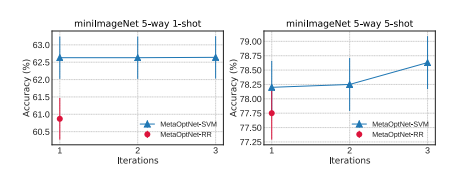
\includegraphics[width=.7\linewidth]{figure/f3.png}
    \caption{使用不同的元训练样本数量,在miniImageNet元测试集上的测试准确率(\%)。}
    \label{fig:3}
\end{figure}
